\section{Methods}
\label{sec:method}

\subsection{Participants}
Thirty right-handed subjects participated in this experiment (twenty-one males; age: 18$-$26 years (mean = 22.2 years; SD = 2.5 years)). All the participants gave informed consent.\\
Participants were primarily found amongst students from the Faculty of Social Sciences at the Radboud University. The following exclusion criteria were used:
\begin{itemize}
	\item Cognitive deficits (or unfamiliarity with the English language) that made comprehension of the information letter and instructions difficult.
	\item Epilepsy. Rapid serial visual presentation uses fast presented stimuli, so this criteria was added as a precaution.
	\item Dyslexia. We used artificial words in the experiment and the participant should have no trouble distinguishing between letters and registering the order of letters.
\end{itemize}

\subsection{Experimental paradigm}
%procedure
The experiment had a between subject design to asses the effect of different reading speeds and exposure time, using three groups:
\begin{enumerate}
	\item \textit{normal}: the task was performed using three times 20 words for training and the stimuli were presented at a normal reading rate of 150 words per minute.
	\item \textit{fast-amount}: the task was performed using three times 20 words for training and the stimuli were presented at a fast presentation rate of 450 words per minute.
	\item \textit{fast-time}: the task was performed using nine times 20 words for training and the stimuli were presented at a fast presentation rate of 450 words per minute.
\end{enumerate}

\noindent In each group were ten participants (\textit{normal}: four males; age: 18$-$26 years (mean = 22 years; SD = 2.4 years), \textit{fast-amount}: nine males; age 19$-$26 years (mean = 22.5 years; SD = 2.5 years), \textit{fast-time}: eight males; age 19$-$26 years (mean = 22.1 years; SD = 2.6 years)).\\
%paradigm \& task
For each group the experiment followed the same structure (shown in Figure \ref{fig:timeline}) and started with a questionnaire. The participant was asked to fill out their age, gender, the number of languages they speak and their experience with speed reading on a scale from 1 (none) to 7 (usage on a regular basis). \\
The participant had to perform three sessions in the experiment. The main task of the experiment is shown in Figure \ref{fig:tasktimeline}). The first session was a practice session to get acquainted with RSVP. The session began with the first three sentences of \textit{Beauty and the Beast}\footnote{\url{http://www.storynory.com/2008/04/28/beauty-and-the-beast-2/}}, at a rate of 150 words per minute. Hereafter, the participant was prompted that the rate would increase to 200 words per minute after a button press. Three to four sentences were presented for each rate, until 500 words per minute was reached.\\
The second session was the training session, which differed between groups. The participants were unaware of differences between groups, and they did not know at which rate the words would be presented, the instructions were the same for all participants and only included that we would use one of the rates presented during practice. The training consisted of three or nine (depending on the condition) takes of 20 words, from the grammar shown in Figure \ref{fig:grammar}. After every take there was time for a break, so the participants would not get too weary to concentrate on the words.

\begin{figure}
\centering
\hspace*{-1.55cm}
\begin{tikzpicture}[shorten >=1pt,node distance=2cm,on grid,auto] 
   \node[state,initial] (S_0)   {$S_0$}; 
   \node[state] (S_1) [above right=of S_0] {$S_1$}; 
   \node[state] (S_2) [below right=of S_0] {$S_2$}; 
   \node[state,accepting] (S_3) [right=of S_1] {$S_3$}; 
   \node[state,accepting] (S_4) [right=of S_2] {$S_4$}; 
   \node[state,accepting](S_5) [below right=of S_3] {$S_5$};
    \path[->] 
    (S_0) edge  node {M} (S_1)
          edge  node [swap] {V} (S_2)
    (S_1) edge  node  {V} (S_3)
          edge [loop above] node {S} ()
    (S_2) edge  node {X} (S_4)
          edge  node {X} (S_1)
    (S_3) edge  node  {R} (S_2)
          edge  node  {S} (S_5)
    (S_4) edge  node  {M} (S_5)
          edge [loop below] node {R} ();
\end{tikzpicture}
\caption{An artificial grammar is given by a finite state machine. States are indicated by circles labeled $S_{i}$. $S_{0}$ is the initial state. Every grammatical item has to start with a transition via an arrow from the initial state to a state directly connected to it (in this case $S_{1}$ or $S_{2}$). States encircled by two lines are final states ($S_{3}$, $S_{4}$, $S_{5}$). The machine can be exited from any final state. The arrows indicate legal transition directions (in this example, it is legal to move from $S_{3}$ to $S_{2}$ but not the other way around). Words are formed by concatenating the letters assigned to each arrow in the order of making the transition (grammatical words are for example MVS, VXRRR).} 
\label{fig:grammar}
\end{figure}
%Insert some figure of an AG with a nice caption explaining how words are formed

\noindent The third session was the test session. The participants were instructed that the words from the training session followed certain rules. Even though they did not learn these rules explicitly, they were asked to answer questions following their `gut feeling'. The participant were then presented with 100 questions, all consisting of a word - either grammatical or nongrammatical - and the question whether they judged the word as grammatical or nongrammatical. There was a total of 50 words, equally many grammatical and nongrammatical words. Each word was represented twice in the questions to check for consistency. The response time and correct response rate were measured. After the task, the participant is asked to fill out a post-questionnaire containing one question: how he decided whether a word was ruleful or unruleful. This was to gain insight in the rules participants used - if any.

\begin{figure}[h]
	\centering
	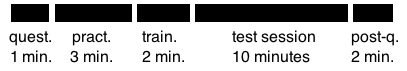
\includegraphics[width=0.45\textwidth]{media/timeline-experiment}
	\caption{This shows the estimated timeline, including small breaks, of the experiment.}
	\label{fig:timeline}
\end{figure}


\begin{figure}[h]
	\centering
	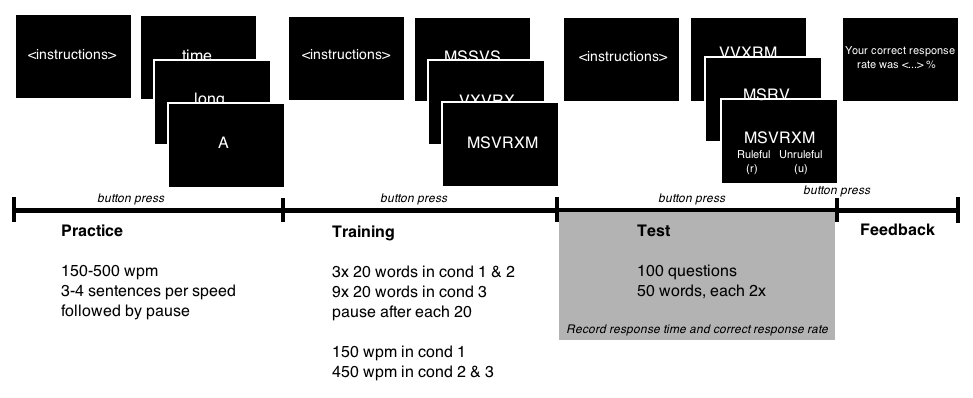
\includegraphics[width=\textwidth]{media/tasktimeline}
	\caption{This figure shows the timeline of the task. The task starts with the welcome screen with instructions about the practice session. The practice session starts at 150 words per minute and after each 3-4 sentences the participant is notified and the speed increases with steps of 50. After practice, instructions for the training session are given and the training starts after a countdown of 3 seconds. During the test session, no feedback is given to ensure that the participants are not learning grammar rules from the test session, only after all questions are answered the correct response rate is given. This concludes the task.}
	\label{fig:tasktimeline}
\end{figure}

\subsection{Materials}
The experiment was done in a soundproof room with a desktop computer.
A program to execute the test as explained earlier was developed in
Python 2.7.8 using the PsychoPy stiumulus generation library
\citep{peirce2008generating}. The stimuli are based on the grammar as
seen in Figure \ref{fig:grammar} and can be found in Table
\ref{tab:stimuli}.

\begin{table}[H]
\centering
\begin{tabular}{p{3.5cm} p{3.5cm} p{3.5cm}}
\toprule
\textbf{Training Items} & \multicolumn{2}{c}{\textbf{Test Items}}\\
\cmidrule(lr{.75em}){1-1}\cmidrule(lr{.75em}){2-3}
grammatical & grammatical & nongrammatical \\
\cmidrule(lr{.75em}){1-1}\cmidrule(lr{.75em}){2-3}
MSSSSV & MSSSV & MMVRX \\
MSSVS & MSSSVS & MSM \\
MSV & MSSV & MSRV \\
MSVRX & MSSVRX & MSRVRX \\ 
MSVRXM & MSV & MSSVSR \\
MVRX & MSVRXR & MSVRSR \\
MVRXRR & MSVRXV & MSVV \\
MVRXSV & MSVS & MXVRXM \\
MVRXV & MVRXM & MXVS \\
MVRXVS & MVRXR & MVRSR \\
VXM & MVRXRM & RRRXV \\
VXRR & MVRXVS & RVS \\
VXRRM & MVS & SSVS \\
VXRRRR & VXR & SVSSXV \\
VXSSVS & VXRM & SXRRM \\
VXSVRX & VXRRR & VRRRM \\
VXSVS & VXRRRM & VVXRM \\
VXVRX & VXSV & VXMRXV \\
VXVRXV & VXSSV & VXRRS \\
VXVS & VXSSSV & VXRS \\
          & VXV & VXRVM \\
         & VXVRX & VXX \\
          & VXVRXR & XRVXV \\
            & VXVRXV & XSSSSV \\
            & VXVS & XVRXRR \\
\bottomrule
\end{tabular}
\caption{Words used for the experiment.}
\label{tab:stimuli}
\end{table}


\subsection{Analysis}
The total number of correct classifications on the 100 test items, $P_{C}$, was determined for each participant. To compare observed to chance level performance for each condition, the one-sample \textit{t}-test (or Wilcoxon signed rank test\footnote{The Shapiro-Wilk test is used to check whether it could be assumed that the samples were drawn from a normally distributed population for each condition. We choose this test because it has the greatest statistical power for small sample sizes \citep{yazici2007comparison}}) will be employed. This will be performed one-tailed because only above chance level performance is of interest.
The 100 items in the testing phase consisted of 50 unique items which were all repeated once. Thus, participants could classify each unique item in one of four ways:
\begin{enumerate}
\item Correct-Correct (CC): classified correctly on both presentations
\item Correct-Erroneous (CE): classified correctly on the first presentation but incorrectly on the second
\item Erroneous-Correct (EC): classified incorrectly on the first presentation but correctly on the second
\item Erroneous-Erroneous (EE): misclassified on both presentations
\end{enumerate}
The sum of CC and EE denotes overall consistency. `When the status of the item is known, it is always classified correctly; when it is not known, a guess is made.' \citep[p.~227]{reber1989implicit}. Using this simple model as a basis, \citeauthor{reber1989implicit} states that CE, EC, and EE should not be statistically distinguishable from each other, since they all reflect guesses. On the other hand, if EE is significantly greater than the average of CE and EC, it can be inferred that judgments were based on rules that are not representative of the grammar. Furthermore, CC should be significantly higher than each of the other three variables if the participants actually implicitly learned a correct, albeit partial, representation of the grammar. Finally, if the difference between CE and EC or EC and CE is significant, it is indicative of forgetting or learning during the testing phase respectively (for an in-depth discussion see \citet{reber1989implicit}). All these measures will be compared to each other using a paired-samples \textit{t}-test. 
Finally, we are interested in seeing whether performance across groups is correlated with the number of languages participants speak or their speed reading experience. To explore this, we will determine Pearson's correlation coefficient for both of these variables.
